\begin{tikzpicture}[draw=gray,color=gray]
    \clip (-17,17) rectangle (17,-3);
    %Xenon
    \filldraw[green] circle (16cm);
    \draw node[scale=4] at (0,14) {$\sigma_a^{^{135}Xe} = 430 kb$};
    %Iodine
    \filldraw[blue!50!] (-9,9) circle (0.1cm);
    \draw node[scale=4] at (-9,7) {$\sigma_a^{^{135}I} = 260 mb$};
    %Uranium
    \filldraw[red!50!] (7,7) circle (0.33cm);
    \draw node[scale=4] at (7,5.5) {$\sigma_f^{^{235}U} = 180 b$};
    %Arrows 
    \draw[->,line width=1mm] (6.5,7) -- (-8.5,9) node[scale=2,midway,above,sloped] {$\gamma_{I} = 6.39\%$};
    \draw[->,line width=1mm] (6.5,7.5) -- (-4,12.5) node[scale=2,midway,above,sloped] {$\gamma_{Xe} = 0.24\%$};
    \draw[->,line width=1mm] (-8.5,9.5) -- (-4.5,12.5) node[scale=2,midway,above,sloped] {$t_{\nicefrac{1}{2}} = 6.7 hr$};
    %Equations
    \draw node[scale=2.5,color=black] at (0,2) {$\frac{dI}{dt} =
    \underbrace{\gamma_{I}\Sigma_{f}^{F}{\phi}(t)}_{\text{Fission Yield}}-\underbrace{\lambda_{I}I(t)}_{\text{Beta Decay}}$};
    \draw node[scale=2.5,color=black] at (0,-1) {$\frac{dXe}{dt} = \underbrace{\lambda_{I}I(t)}_{\text{Precursor Decay}}+\underbrace{\gamma_{Xe}\Sigma_{f}^{F}{\phi}(t)}_{\text{Fission Yield}}-\underbrace{\lambda_{Xe}Xe(t)}_{\text{Beta Decay}}-\underbrace{Xe(t)\sigma_{a}^{Xe}{\phi}(t)}_{\text{Radiative Capture}}$};
\end{tikzpicture}

